\begin{frame}{Master Motor (Left)}
  \framesubtitle{Setpoint characteristics}
	\begin{itemize}
		\item Winds the metal strip
		\item Higher velocity than feeding motor due to elongation
	\end{itemize}
  \centering
  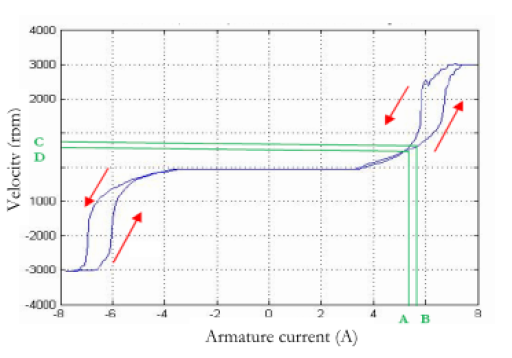
\includegraphics[height=0.6\textheight]{LM_RPM_Current.png}

	\end{frame}

\begin{frame}{Master Motor}
  \framesubtitle{Identification}
  $LM(s) \simeq \frac{5.398}{3.642S+1}$
	\centering
	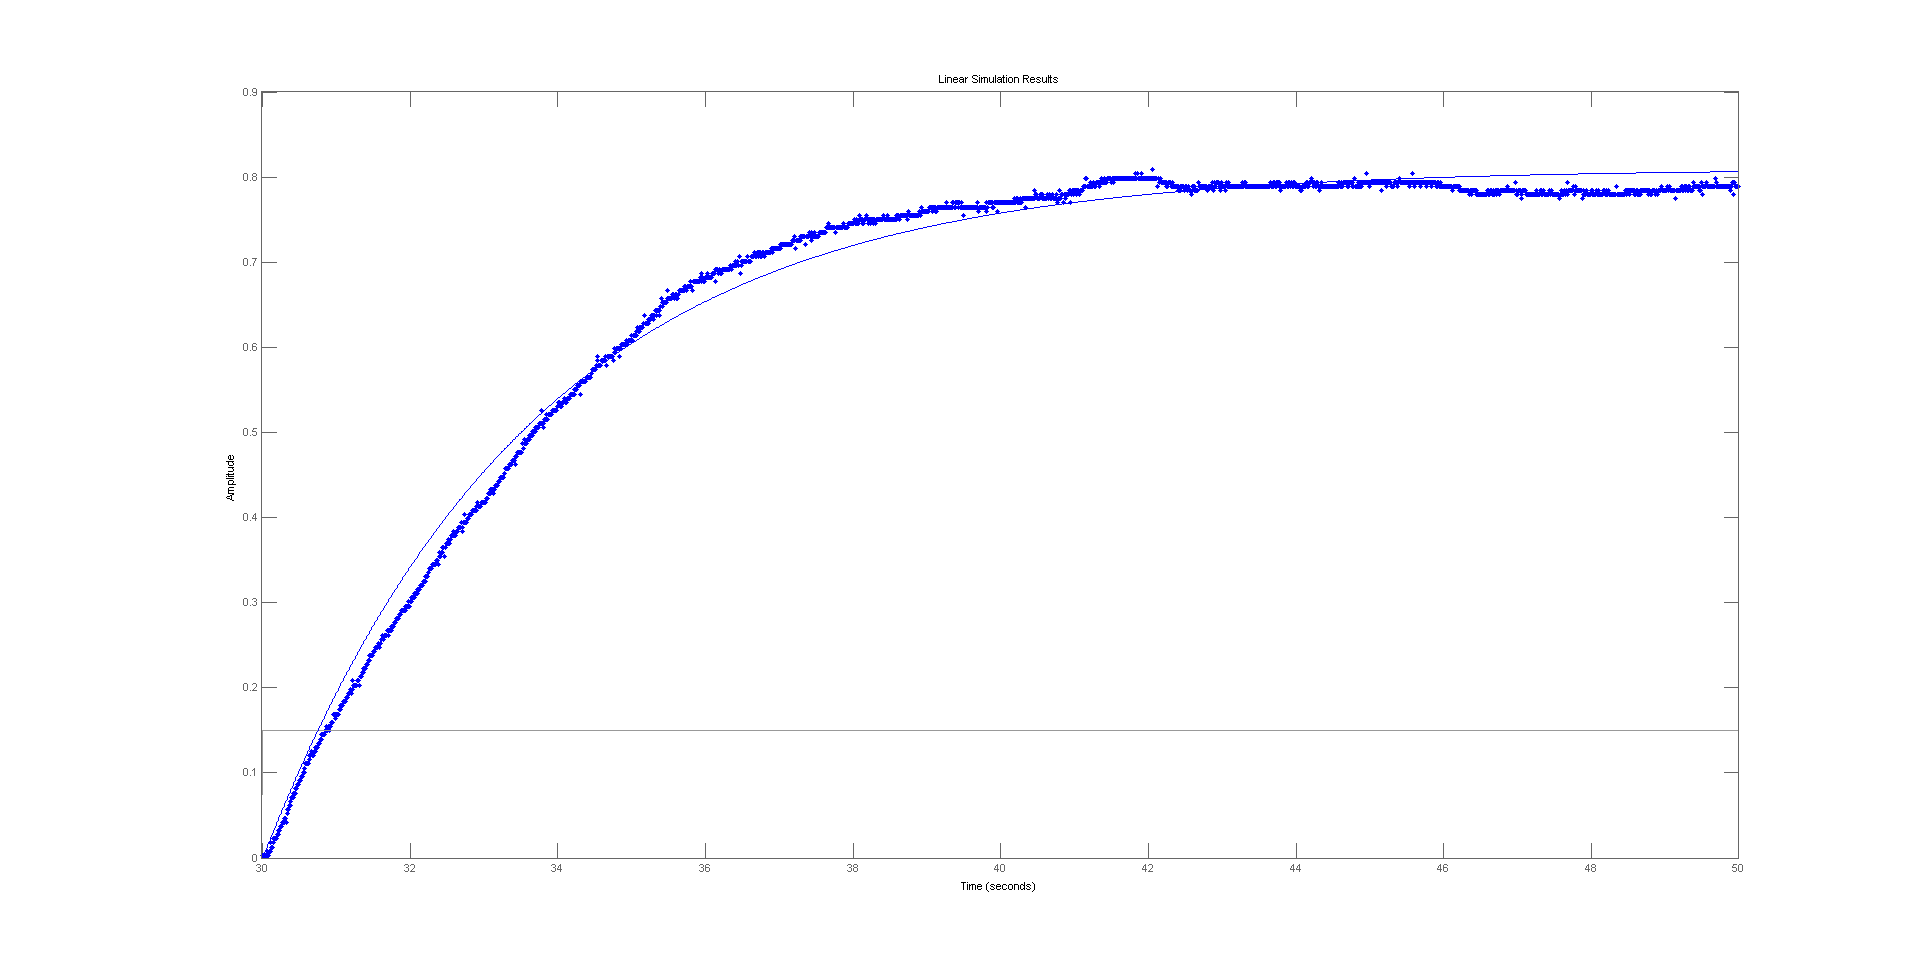
\includegraphics[width=1.00\textwidth]{identification_step_setpoints.png}
\end{frame}

\begin{frame}{Master Motor}
  \framesubtitle{Controller Choice}
\begin{block}{PI Controller}
	\begin{itemize}
		\item Zero steady state error
		\item Disturbance rejection
	\end{itemize}
  \begin{align*}
  LM(s) &= \frac{1.482}{s+0.274}\\
  PI(s) &= K_p + \frac{K_i}{s}\\
        &= K_p \cdot \frac{s+\frac{K_i}{K_p}}{s}
\end{align*}
\end{block}
\end{frame}

\begin{frame}{Master Motor}
\framesubtitle{Controller Tuning}
\begin{itemize}
\item $\frac{K_i}{K_p} =$ chosen at $0.294$ to cancel plant pole
\item $OL(s) = \frac{1.482}{s}$
\end{itemize}
\centering
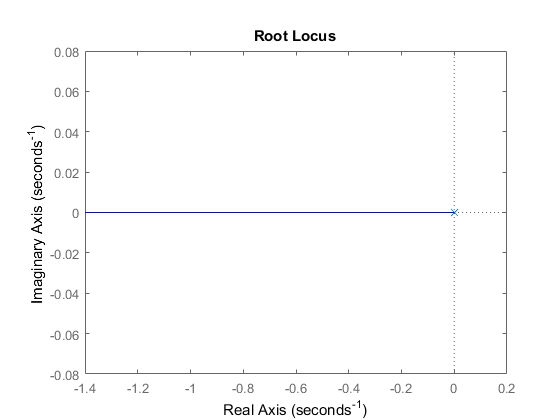
\includegraphics[height=0.6\textheight]{LM_cont_rlocus.png}
\end{frame}



	\begin{frame}{Master Motor}
\framesubtitle{Simulation -- $K_P = 2$}

\centering
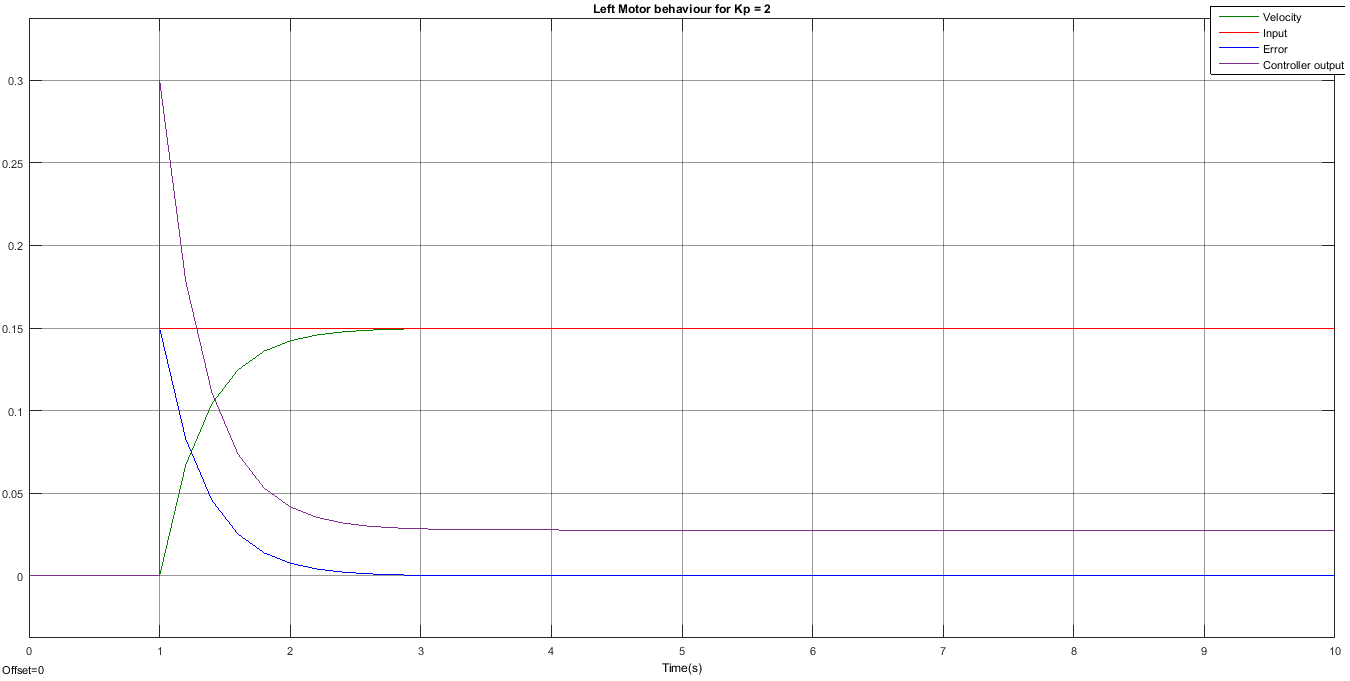
\includegraphics[width = \textwidth]{LM_KP200_sim.png}
\end{frame}




\begin{frame}{Master Motor}
\framesubtitle{Verification}
\centering
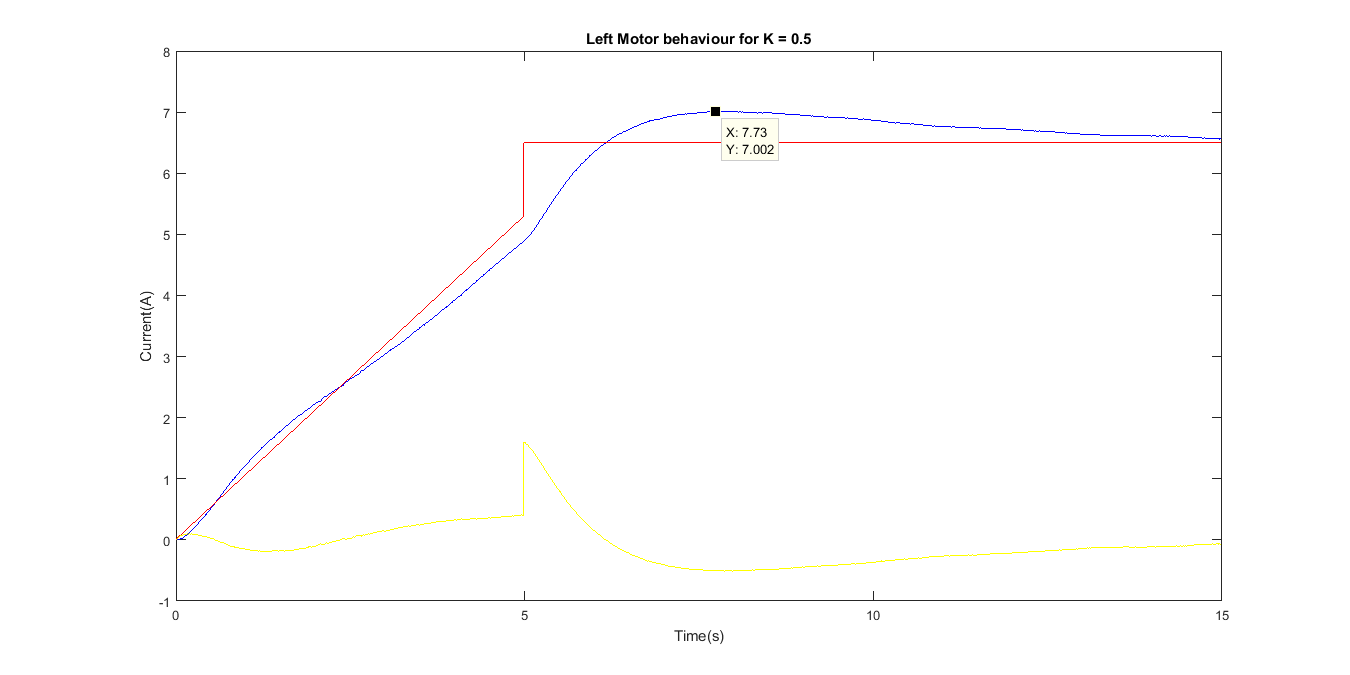
\includegraphics[width = \textwidth]{LM_KP050.png}
\end{frame}


\begin{frame}{Master Motor}
\framesubtitle{Verification}
\centering
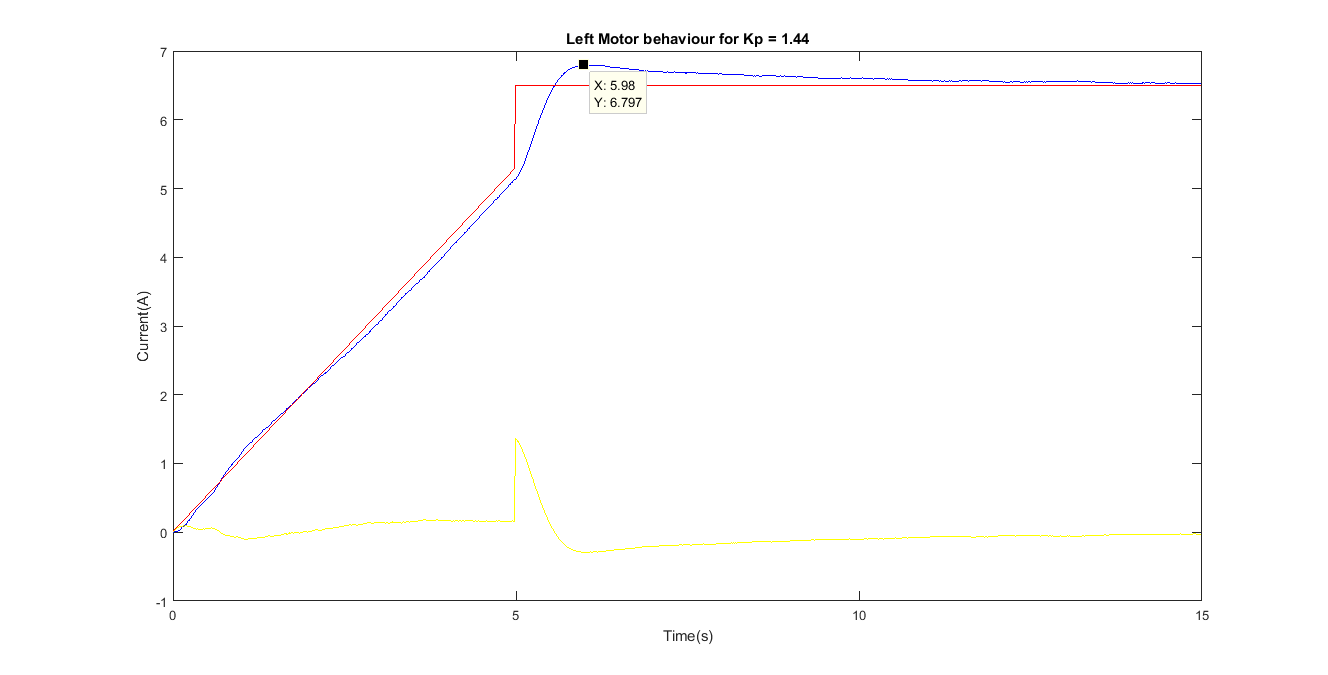
\includegraphics[width = \textwidth]{LM_KP144.png}
\end{frame}


\begin{frame}{Master Motor}
\framesubtitle{Verification}
\centering
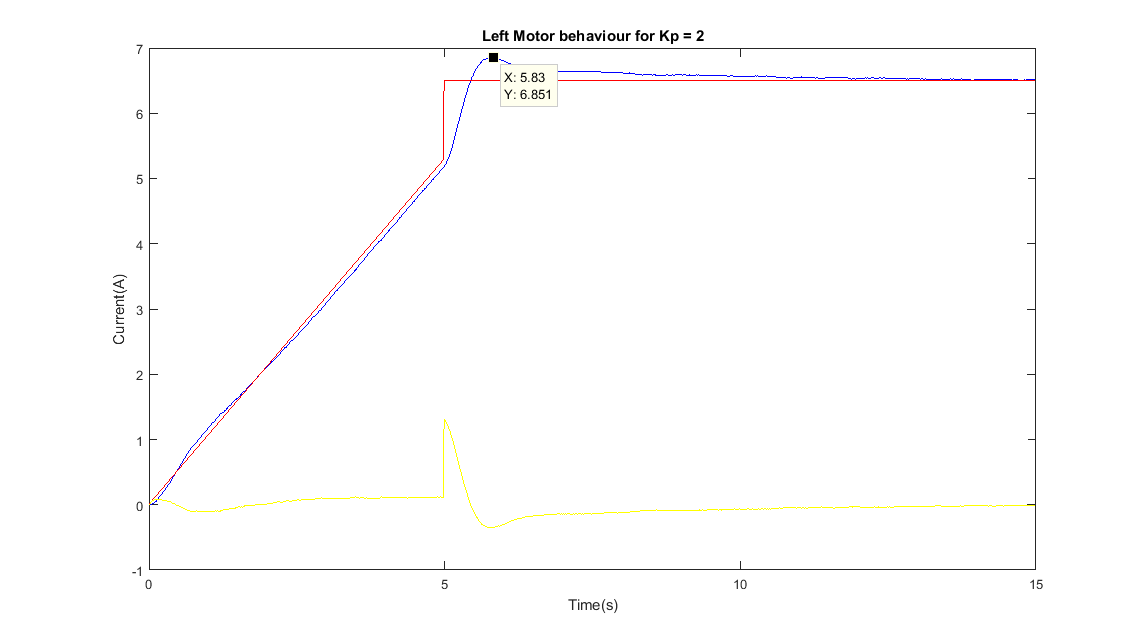
\includegraphics[width = \textwidth]{LM_KP200.png}
\end{frame}

\begin{frame}{Master Motor}
\framesubtitle{Conclusion}
\begin{itemize}
\item PI Controller for zero steady state error
\item Gain $K_P = 2$, $K_I = 0.588$ chosen for quickest settling time, reasonable overshoot
\item Overshoot is due to non linearities and higher order effects
\end{itemize}
\end{frame}
